% SPDX-FileCopyrightText: © 2026 Idiap Research Institute <contact@idiap.ch>
%
% SPDX-FileContributor: Andre Freitas <andre.freitas@idiap.ch>
% Neuro-symbolic AI Group
%
% SPDX-FileContributor: Danilo Gusicuma <danilo.gusicuma@idiap.ch>
% Neuro-symbolic AI Group
%
% SPDX-License-Identifier: MIT
\documentclass[11pt]{article}

\usepackage[margin=1in]{geometry}
\usepackage[T1]{fontenc}
\usepackage[utf8]{inputenc}
\usepackage{lmodern}
\usepackage{microtype}
\usepackage{amsmath,amssymb,amsthm,mathtools}
\usepackage{enumitem}
\usepackage{booktabs,tabularx,array}
\usepackage{hyperref}
\usepackage{xcolor}
\usepackage{tikz}
\usetikzlibrary{arrows.meta,calc}

\hypersetup{
  colorlinks=true,
  linkcolor=blue!50!black,
  citecolor=blue!50!black,
  urlcolor=blue!50!black,
  pdftitle={A Finite Schur--Feshbach Test for Reflected Wilson Blocks: An Explicit Four-Dimensional SU(2) Heat-Kernel Lattice Realization},
  pdfauthor={Andre Freitas},
  pdfsubject={Finite reflection-positivity certificates for Wilson blocks}
}

\newtheorem{theorem}{Theorem}[section]
\newtheorem{lemma}[theorem]{Lemma}
\newtheorem{proposition}[theorem]{Proposition}
\newtheorem{corollary}[theorem]{Corollary}
\newtheorem{definition}[theorem]{Definition}
\newtheorem{remark}[theorem]{Remark}
\newtheorem{assumption}[theorem]{Assumption}

\newcommand{\one}{\mathbf 1}
\newcommand{\C}{\mathbb C}
\newcommand{\R}{\mathbb R}
\newcommand{\eps}{\varepsilon}
\newcommand{\norm}[1]{\lVert #1\rVert}
\newcommand{\Span}{\operatorname{span}}
\newcommand{\Ker}{\operatorname{Ker}}
\newcommand{\Ran}{\operatorname{Ran}}
\newcommand{\diag}{\operatorname{diag}}
\newcommand{\Herm}{\operatorname{Herm}}
\newcommand{\OS}{\mathrm{OS}}
\newcommand{\HK}{\mathrm{HK}}
\newcommand{\Had}{\circ}
\newcommand{\odiv}{\oslash}
\newcommand{\Tr}{\operatorname{Tr}}
\newcommand{\Rea}{\operatorname{Re}}

\newenvironment{openmodule}[1]
{\begin{quote}\color{red!55!black}\textbf{Open module #1.}\ }
{\end{quote}}

\title{A Finite Schur--Feshbach Test for Reflected Wilson Blocks:\\
An Explicit Four-Dimensional \texorpdfstring{$SU(2)$}{SU(2)} Heat-Kernel Lattice Realization}
\author{Andre Freitas\\[2pt]\small\textit{Affiliation and contact information to be supplied}}
\date{July 10, 2026}

\begin{document}
\maketitle

\begin{abstract}
We give a fully specified finite-cutoff realization of a Schur--Feshbach positivity test for reflected Wilson observables.  The matrix statement is the rank-one specialization of standard second-order geometry of the positive-semidefinite cone: if
\[
q_\eps=\one\one^*+\eps H+\eps^2K+o(\eps^2),
\]
then, after eliminating the rank-one direction, the first two coefficients are
\[
A=PHP,
\qquad
C=P\bigl(K-n^{-1}Hee^*H\bigr)P,
\qquad
e=n^{-1/2}\one,
\quad P=I-ee^*.
\]
The field-theoretic contribution is an explicit same-theory block.  On a finite four-dimensional reflection-symmetric lattice with gauge group $SU(2)$ and heat-kernel plaquette weight, we define three closed hairpin loops sharing a base path.  A spatial-reflection odd Wilson mode $X$ and an even centered Wilson mode $Y$ generate three positive-time observables
\[
F_i^\eps=1+\sqrt\eps\,b_iX+\eps c_iY,
\qquad
b=(1,-1,0)^T,
\quad c=(0,0,1)^T.
\]
Their reflected Gram matrix is exactly
\[
N_\eps=\one\one^T+\eps\sigma bb^T+\eps^2\tau cc^T,
\qquad
\sigma=\langle\Theta X,X\rangle_{\OS}\ge0,
\quad
\tau=\langle\Theta Y,Y\rangle_{\OS}\ge0.
\]
Diagonal correlation normalization is realized by rescaling the same observables, hence is an exact congruence rather than an uncontrolled entrywise quotient.  The normalized block has a rank-one limit and yields
\[
PHP=\sigma bb^T,
\qquad
C=-\sigma^2bb^T+\frac{\tau}{9}zz^T,
\qquad z=(1,1,-2)^T.
\]
Thus the first reduced eigenvalue is $2\sigma$, while the corrected second-order null-sector eigenvalue is $2\tau/3$.  The uncorrected quantity contains a spurious $\sigma^2$ term, which the Schur--Feshbach correction removes.  All statements up to this point are exact at finite cutoff.  Geometric collar collapse, uniform nondegeneracy along a continuum trajectory, endpoint cumulant estimates, infinite volume, and a spectral-gap implication are isolated as explicit open modules rather than claimed results.
\end{abstract}

\tableofcontents

\section{Scope, novelty, and claim boundary}

The Yang--Mills existence and mass-gap problem asks for a nontrivial four-dimensional quantum Yang--Mills theory for every compact simple gauge group and a positive mass gap in the same reconstructed theory \cite{JaffeWitten2000,ClayYM}.  Osterwalder--Schrader reconstruction provides a Euclidean route, in which reflection positivity is one indispensable axiom \cite{OsterwalderSchrader1973,OsterwalderSchrader1975}.  At finite lattice spacing, standard plaquette gauge actions furnish reflection-positive regulated theories \cite{OsterwalderSeiler1978,Luscher1977}.

This paper makes a deliberately narrower contribution.  It does not construct a continuum Yang--Mills measure, establish all OS axioms, prove exponential clustering, or prove a mass gap.  It does two finite things:

\begin{enumerate}[label=(\roman*)]
  \item it states the rank-one Schur--Feshbach coefficient test for a singular PSD matrix family; and
  \item it implements that test on an explicit four-dimensional $SU(2)$ lattice Wilson block whose action, reflection, observables, normalization, rank-one limit, coefficients, and finite margins are all specified.
\end{enumerate}

The Schur-complement curvature term is not presented as a new discovery in matrix analysis.  It is a rank-one instance of the established second-order geometry of semidefinite constraints \cite{Shapiro1997,BonnansShapiro2000}.  The purpose of retaining the finite theorem is to make the Wilson calculation self-contained and to show exactly where the curvature correction enters.  The substantive advance over a purely schematic Wilson/OS discussion is the same-theory realization in Sections \ref{sec:lattice-model}--\ref{sec:finite-certificate}.

\paragraph{Claim boundary.}
All results through Corollary \ref{cor:implemented-route-a} hold on a fixed finite lattice, and the source-collision expansion is uniform over arbitrary cutoff families because the primitive Wilson observables are bounded.  Strict positive margins require the finite nondegeneracy conditions $\sigma>0$ and $\tau>0$.  No uniform lower bound on these quantities as the cutoff is removed is proved here.

\section{Finite reflected Gram matrices and the Schur--Feshbach test}
\label{sec:finite-theorem}

Let $\Theta$ be an antilinear Euclidean reflection and let $\mathcal A_+$ be an algebra of positive-time observables.  Reflection positivity means
\begin{equation}
  \sum_{i,j=1}^n\overline{c_i}c_j
  \left\langle (\Theta F_i)^*F_j\right\rangle\ge0
  \label{eq:os-positivity}
\end{equation}
for every finite family $F_1,\ldots,F_n\in\mathcal A_+$ and every $c\in\C^n$.  Equivalently, the reflected Gram matrix
\begin{equation}
  N_{ij}=\left\langle (\Theta F_i)^*F_j\right\rangle
  \label{eq:gram-general}
\end{equation}
is positive semidefinite.

Suppose a normalized finite block has a rank-one collision expansion
\begin{equation}
  q_\eps=\one\one^*+\eps H+\eps^2K+R_\eps,
  \qquad
  \norm{R_\eps}=o(\eps^2),
  \label{eq:rank-one-expansion}
\end{equation}
where $H,K\in\Herm_n(\C)$.  Define
\begin{equation}
  e=n^{-1/2}\one,
  \qquad
  P=I-ee^*.
  \label{eq:e-P}
\end{equation}
Then $P$ projects onto $\one^\perp$ and $\one\one^*=nee^*$.

\begin{theorem}[Rank-one Schur--Feshbach certificate]
\label{thm:schur-feshbach}
Let $q_\eps$ satisfy \eqref{eq:rank-one-expansion}.  Set
\begin{equation}
  \lambda_\eps=e^*q_\eps e,
  \qquad
  \mathcal F_\eps
  =Pq_\eps P-Pq_\eps e\,\lambda_\eps^{-1}e^*q_\eps P.
  \label{eq:feshbach-map}
\end{equation}
For all sufficiently small $\eps>0$, $\lambda_\eps>0$ and
\begin{equation}
  q_\eps\succeq0
  \quad\Longleftrightarrow\quad
  \mathcal F_\eps\succeq0.
  \label{eq:schur-equivalence}
\end{equation}
Moreover,
\begin{equation}
  \mathcal F_\eps
  =\eps A+\eps^2C+o(\eps^2),
  \qquad
  A=PHP,
  \qquad
  C=P\bigl(K-n^{-1}Hee^*H\bigr)P.
  \label{eq:A-C-general}
\end{equation}
If $q_\eps\succeq0$ for all sufficiently small $\eps>0$, then
\begin{equation}
  A\succeq0\quad\text{on }\one^\perp,
  \label{eq:A-positive}
\end{equation}
and, writing $\Pi$ for the orthogonal projection onto $\Ker A\subset\one^\perp$,
\begin{equation}
  \Pi C\Pi\succeq0\quad\text{on }\Ker A.
  \label{eq:C-positive}
\end{equation}
\end{theorem}

\begin{proof}
Since $q_0=nee^*$,
\[
  \lambda_\eps=n+\eps e^*He+O(\eps^2)>0
\]
for small $\eps$.  With respect to $\C^n=\C e\oplus P\C^n$, the usual scalar Schur complement gives \eqref{eq:schur-equivalence}.  Furthermore,
\begin{align*}
  Pq_\eps P&=\eps PHP+\eps^2PKP+o(\eps^2),\\
  Pq_\eps e&=\eps PHe+\eps^2PKe+o(\eps^2),\\
  \lambda_\eps^{-1}&=n^{-1}+O(\eps).
\end{align*}
Hence
\[
  Pq_\eps e\,\lambda_\eps^{-1}e^*q_\eps P
  =\eps^2n^{-1}PHee^*HP+o(\eps^2),
\]
which proves \eqref{eq:A-C-general}.  If $\mathcal F_\eps\succeq0$, then for $v\in\one^\perp$,
\[
  0\le v^*\mathcal F_\eps v
  =\eps v^*Av+\eps^2v^*Cv+o(\eps^2).
\]
Division first by $\eps$, and then by $\eps^2$ on $\Ker A$, gives \eqref{eq:A-positive} and \eqref{eq:C-positive}.
\end{proof}

\begin{remark}[The curvature correction]
Since $ee^*=n^{-1}\one\one^*$,
\begin{equation}
  C=PKP-n^{-2}PH\one\one^*HP.
  \label{eq:C-one}
\end{equation}
The second term is the excursion from $\one^\perp$ into the rank-one direction and back.  Replacing $C$ by $PKP$ generally changes the null-sector value.
\end{remark}

\begin{proposition}[Strict second-order sufficiency]
\label{prop:strict-sufficiency}
Assume $A\succeq0$ on $\one^\perp$.  Let $\Pi$ project onto $\Ker A$ and put $Q=P-\Pi$.  If, for some $\alpha,\beta>0$,
\begin{equation}
  QAQ\succeq\alpha Q,
  \qquad
  \Pi C\Pi\succeq\beta\Pi,
  \label{eq:strict-margins}
\end{equation}
then $q_\eps\succeq0$ for all sufficiently small $\eps>0$.
\end{proposition}

\begin{proof}
On $Q\C^n$, $Q\mathcal F_\eps Q=\eps QAQ+O(\eps^2)$ is positive and has inverse of order $O(\eps^{-1})$.  Because $A\Pi=0=\Pi A$, the off-diagonal block $\Pi\mathcal F_\eps Q$ is $O(\eps^2)$.  The Schur complement on $\Pi\C^n$ is therefore
\[
  \eps^2\Pi C\Pi+o(\eps^2)-O(\eps^3),
\]
which is positive for small $\eps$ by \eqref{eq:strict-margins}.  Theorem \ref{thm:schur-feshbach} then gives $q_\eps\succeq0$.
\end{proof}

\begin{remark}[Higher-order recursion requires higher-order data]
The two-order hypothesis \eqref{eq:rank-one-expansion} supports only the two tests above.  A recursive null-sector procedure is justified only when an asymptotic expansion through the required order, or analyticity in $\eps$, is available.  An $o(\eps^2)$ remainder alone does not determine the next sign.
\end{remark}

\section{A reflection-positive four-dimensional lattice model}
\label{sec:lattice-model}

\subsection{Finite lattice, action, and reflections}

Fix a lattice spacing $a>0$, integers $T,L\ge1$, and the finite reflection-symmetric lattice
\begin{equation}
  \Lambda_{T,L}
  =\{-T+1,\ldots,T\}\times(\mathbb Z/L\mathbb Z)^3.
  \label{eq:lattice}
\end{equation}
The first coordinate is Euclidean time.  An oriented nearest-neighbour edge $\ell$ carries a link variable $U_\ell\in SU(2)$, with $U_{\bar\ell}=U_\ell^{-1}$.  For a plaquette $p$, $U_p$ is the ordered product of link variables around its boundary.

Let $K_\kappa$ be the $SU(2)$ heat kernel at time $\kappa>0$, in the convention
\begin{equation}
  K_\kappa(g)
  =\sum_{j\in\frac12\mathbb N_0}
  (2j+1)e^{-\kappa j(j+1)}\chi_j(g).
  \label{eq:heat-kernel}
\end{equation}
The finite-volume heat-kernel plaquette measure is
\begin{equation}
  d\mu_{\Lambda,\kappa}(U)
  =Z_{\Lambda,\kappa}^{-1}
  \left(\prod_{\ell}dU_\ell\right)
  \left(\prod_p K_\kappa(U_p)\right),
  \label{eq:hk-measure}
\end{equation}
where $dU_\ell$ is normalized Haar measure.  This is a finite-dimensional probability measure.  The heat-kernel action is a standard lattice Yang--Mills action and has strictly positive character coefficients \cite{MenottiOnofri1981}.

Reflect the lattice through the link plane $t=\tfrac12$:
\begin{equation}
  \vartheta(t,x_1,x_2,x_3)=(1-t,x_1,x_2,x_3).
  \label{eq:time-reflection}
\end{equation}
The induced antilinear operation on observables is denoted by $\Theta$.  Let $\mathcal A_+$ be the gauge-invariant Wilson algebra generated by loops whose links lie entirely in the positive half $t\ge1$.

\begin{proposition}[Finite reflection positivity]
\label{prop:lattice-rp}
For the measure \eqref{eq:hk-measure},
\begin{equation}
  \left\langle(\Theta F)^*F\right\rangle_{\Lambda,\kappa}\ge0
  \qquad(F\in\mathcal A_+).
  \label{eq:lattice-rp}
\end{equation}
Consequently every finite reflected Wilson Gram matrix is positive semidefinite.
\end{proposition}

\begin{proof}[Justification]
This is the standard link-reflection positivity theorem for plaquette gauge actions with nonnegative character coefficients \cite{OsterwalderSeiler1978,Luscher1977}.  In the heat-kernel case the coefficients in \eqref{eq:heat-kernel} are positive.  The Peter--Weyl expansion factorizes each plaquette crossing the reflection plane into a sum of reflected products with nonnegative weights; plaquettes entirely on one side occur in reflected pairs.  Expanding the finite product and integrating gives \eqref{eq:lattice-rp}.
\end{proof}

We also use the spatial reflection
\begin{equation}
  \rho(t,x_1,x_2,x_3)=(t,x_1,-x_2,x_3).
  \label{eq:rho}
\end{equation}
The measure is invariant under $\rho$, and $\rho$ commutes with $\vartheta$.

\subsection{Three explicit closed hairpins}
\label{sec:hairpin-geometry}

Let $e_0,e_1,e_2,e_3$ be the lattice unit vectors, with $e_0$ temporal.  Choose positive integers $r,s,h$ so that the following paths do not wrap around the finite box.  Put
\[
  A=(1,0,0,0),
  \qquad
  B=A+re_1,
\]
and let $\beta$ be the straight path from $A$ to $B$.  Define three detours from $A$ to $B$:
\begin{align}
  \eta_+&:
  A\longrightarrow A+se_2
  \longrightarrow B+se_2
  \longrightarrow B,
  \label{eq:eta-plus}\\
  \eta_-&:
  A\longrightarrow A-se_2
  \longrightarrow B-se_2
  \longrightarrow B,
  \label{eq:eta-minus}\\
  \eta_0&:
  A\longrightarrow A+he_0
  \longrightarrow B+he_0
  \longrightarrow B.
  \label{eq:eta-zero}
\end{align}
The closed hairpin loops are
\begin{equation}
  \gamma_\alpha=\eta_\alpha\circ\beta^{-1},
  \qquad \alpha\in\{+,-,0\}.
  \label{eq:gamma-hairpins}
\end{equation}
All links lie in $t\ge1$.  The loops share the base path $\beta$, and
\begin{equation}
  \rho\gamma_+=\gamma_-,
  \qquad
  \rho\gamma_0=\gamma_0.
  \label{eq:rho-loops}
\end{equation}

\begin{figure}[t]
\centering
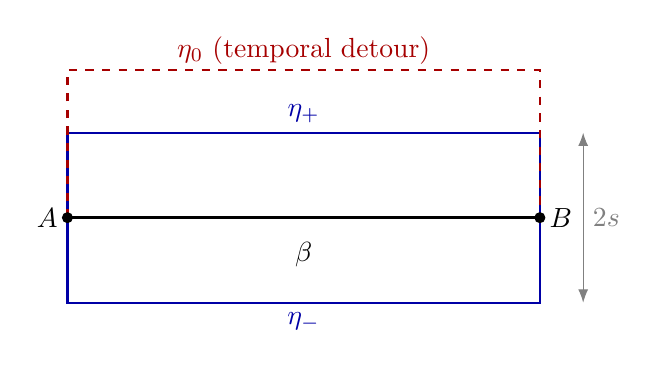
\begin{tikzpicture}[x=1.0cm,y=0.8cm,>=Latex]
  \coordinate (A) at (0,0);
  \coordinate (B) at (6,0);
  \draw[very thick] (A)--(B) node[midway,below=5pt] {$\beta$};
  \draw[blue!65!black,thick] (A)--(0,1.35)--(6,1.35)--(B);
  \draw[blue!65!black,thick] (A)--(0,-1.35)--(6,-1.35)--(B);
  \draw[red!65!black,dashed,thick] (A)--(0,2.35)--(6,2.35)--(B);
  \fill (A) circle (2pt) node[left] {$A$};
  \fill (B) circle (2pt) node[right] {$B$};
  \node[blue!65!black] at (3,1.65) {$\eta_+$};
  \node[blue!65!black] at (3,-1.65) {$\eta_-$};
  \node[red!65!black] at (3,2.65) {$\eta_0$ (temporal detour)};
  \draw[<->,gray] (6.55,-1.35)--(6.55,1.35) node[midway,right] {$2s$};
\end{tikzpicture}
\caption{Schematic projection of the three detours.  The dashed detour $\eta_0$ lies in the Euclidean-time direction; the picture only displays the shared-base incidence pattern.}
\label{fig:hairpins}
\end{figure}

For a closed path $\gamma$, define the normalized fundamental Wilson loop
\begin{equation}
  W_\gamma(U)=\frac12\Tr U_\gamma.
  \label{eq:Wilson-loop}
\end{equation}
For $SU(2)$ this is real and lies in $[-1,1]$.  Write $W_+=W_{\gamma_+}$, $W_-=W_{\gamma_-}$, and $W_0=W_{\gamma_0}$.  Define
\begin{equation}
  X=\frac12(W_+-W_-),
  \qquad
  Y=W_0-m_0,
  \qquad
  m_0=\langle W_0\rangle_{\Lambda,\kappa}.
  \label{eq:X-Y}
\end{equation}
Then $X,Y\in\mathcal A_+$, $|X|\le1$, $|Y|\le2$, and
\begin{equation}
  \rho X=-X,
  \qquad
  \rho Y=Y,
  \qquad
  \langle X\rangle=\langle Y\rangle=0.
  \label{eq:parities}
\end{equation}

\begin{lemma}[Symmetry decoupling]
\label{lem:symmetry-decoupling}
The mixed reflected correlations vanish:
\begin{equation}
  \left\langle(\Theta X)Y\right\rangle_{\Lambda,\kappa}=0,
  \qquad
  \left\langle(\Theta Y)X\right\rangle_{\Lambda,\kappa}=0.
  \label{eq:mixed-zero}
\end{equation}
\end{lemma}

\begin{proof}
Because the measure is $\rho$-invariant and $\rho$ commutes with $\Theta$,
\[
  \langle(\Theta X)Y\rangle
  =\langle(\Theta\rho X)(\rho Y)\rangle
  =-\langle(\Theta X)Y\rangle.
\]
Thus the first correlation is zero.  The second is its Hermitian conjugate and also vanishes.
\end{proof}

\section{The exact three-hairpin source block}
\label{sec:exact-block}

\subsection{Positive-time observables and exact Gram matrix}

Let
\begin{equation}
  b=(1,-1,0)^T,
  \qquad
  c=(0,0,1)^T,
  \qquad
  z=(1,1,-2)^T.
  \label{eq:b-c-z}
\end{equation}
Thus $b\perp\one$, $z\perp\one$, and $b\perp z$.  For $\eps\ge0$, define three observables in the same positive-time Wilson algebra:
\begin{equation}
  F_i^\eps
  =1+\sqrt\eps\,b_iX+\eps c_iY,
  \qquad i=1,2,3.
  \label{eq:F-source-family}
\end{equation}
The square root appears only at the observable level.  The $\rho$ parity in Lemma \ref{lem:symmetry-decoupling} removes half-integer powers from the Gram matrix.

Set
\begin{equation}
  \sigma
  =\left\langle(\Theta X)X\right\rangle_{\Lambda,\kappa},
  \qquad
  \tau
  =\left\langle(\Theta Y)Y\right\rangle_{\Lambda,\kappa}.
  \label{eq:sigma-tau}
\end{equation}
By Proposition \ref{prop:lattice-rp},
\begin{equation}
  0\le\sigma\le1,
  \qquad
  0\le\tau\le4.
  \label{eq:sigma-tau-bounds}
\end{equation}
The upper bounds follow from $|X|\le1$ and $|Y|\le2$.

\begin{proposition}[Exact reflected Gram block]
\label{prop:exact-N}
The reflected Gram matrix
\begin{equation}
  N_\eps(i,j)
  =\left\langle(\Theta F_i^\eps)^*F_j^\eps\right\rangle_{\Lambda,\kappa}
  \label{eq:N-definition}
\end{equation}
is exactly
\begin{equation}
  N_\eps
  =\one\one^T+\eps\sigma bb^T+\eps^2\tau cc^T.
  \label{eq:N-exact}
\end{equation}
In particular, $N_\eps\succeq0$ for every $\eps\ge0$.
\end{proposition}

\begin{proof}
Expanding \eqref{eq:N-definition}, the one-point terms vanish by \eqref{eq:parities}.  The order-$\eps^{3/2}$ mixed terms vanish by \eqref{eq:mixed-zero}.  The remaining terms are precisely those in \eqref{eq:N-exact}; there are no higher terms because \eqref{eq:F-source-family} is polynomial of degree one in $\sqrt\eps X$ and degree one in $\eps Y$.  Positivity also follows directly from
\[
  v^TN_\eps v
  =|\one^Tv|^2+\eps\sigma|b^Tv|^2+\eps^2\tau|c^Tv|^2.
\]
\end{proof}

\subsection{Same-theory correlation normalization}

The diagonal entries of \eqref{eq:N-exact} are
\begin{equation}
  N_{11}=N_{22}=1+\eps\sigma,
  \qquad
  N_{33}=1+\eps^2\tau.
  \label{eq:N-diagonal}
\end{equation}
Define
\begin{equation}
  D_\eps
  =\diag\left(
  (1+\eps\sigma)^{-1/2},
  (1+\eps\sigma)^{-1/2},
  (1+\eps^2\tau)^{-1/2}
  \right)
  \label{eq:D-normalization}
\end{equation}
and normalized observables
\begin{equation}
  \widetilde F_i^\eps=(D_\eps)_{ii}F_i^\eps.
  \label{eq:normalized-observables}
\end{equation}
Their reflected Gram matrix is
\begin{equation}
  q_\eps=D_\eps N_\eps D_\eps,
  \qquad
  (q_\eps)_{ij}
  =\frac{N_\eps(i,j)}{\sqrt{N_\eps(i,i)N_\eps(j,j)}}.
  \label{eq:q-congruence}
\end{equation}
This is an exact observable-level congruence.  It is therefore positivity preserving and does not invoke an arbitrary pair-dependent quotient.

\begin{proposition}[Exact normalized block]
\label{prop:exact-q}
The normalized matrix is
\begin{equation}
  q_\eps=
  \begin{pmatrix}
  1&\alpha_\eps&\beta_\eps\\
  \alpha_\eps&1&\beta_\eps\\
  \beta_\eps&\beta_\eps&1
  \end{pmatrix},
  \label{eq:q-exact}
\end{equation}
where
\begin{equation}
  \alpha_\eps=\frac{1-\eps\sigma}{1+\eps\sigma},
  \qquad
  \beta_\eps=\frac{1}{\sqrt{(1+\eps\sigma)(1+\eps^2\tau)}}.
  \label{eq:alpha-beta}
\end{equation}
It satisfies $q_\eps\succeq0$ for every $\eps\ge0$ and
\begin{equation}
  q_\eps\longrightarrow\one\one^T
  \qquad(\eps\downarrow0).
  \label{eq:q-rank-one-limit}
\end{equation}
If $\sigma>0$ and $\tau>0$, then $q_\eps\succ0$ for every $\eps>0$, and
\begin{equation}
  \det q_\eps
  =\frac{4\eps^3\sigma\tau}
  {(1+\eps\sigma)^2(1+\eps^2\tau)}.
  \label{eq:q-determinant}
\end{equation}
\end{proposition}

\begin{proof}
Equations \eqref{eq:q-exact}--\eqref{eq:alpha-beta} follow from \eqref{eq:N-exact} and \eqref{eq:D-normalization}.  Positivity and the rank-one limit follow from the congruence \eqref{eq:q-congruence}.  If $\sigma,\tau>0$ and $\eps>0$, the three linear functionals $\one^Tv$, $b^Tv$, and $c^Tv$ separate points of $\R^3$, so \eqref{eq:N-exact} is positive definite.  Direct calculation gives \eqref{eq:q-determinant}.
\end{proof}

\section{Coefficient extraction and the finite certificate}
\label{sec:finite-certificate}

Expanding \eqref{eq:alpha-beta} at $\eps=0$ gives
\begin{align}
  \alpha_\eps
  &=1-2\sigma\eps+2\sigma^2\eps^2+O(\eps^3),
  \label{eq:alpha-expansion}\\
  \beta_\eps
  &=1-\frac{\sigma}{2}\eps
  +\left(\frac{3\sigma^2}{8}-\frac{\tau}{2}\right)\eps^2
  +O(\eps^3).
  \label{eq:beta-expansion}
\end{align}
Thus
\begin{equation}
  q_\eps=\one\one^T+\eps H+\eps^2K+R_\eps,
  \label{eq:q-HK}
\end{equation}
with
\begin{equation}
H=
\begin{pmatrix}
0&-2\sigma&-\sigma/2\\
-2\sigma&0&-\sigma/2\\
-\sigma/2&-\sigma/2&0
\end{pmatrix}
\label{eq:H-explicit}
\end{equation}
and
\begin{equation}
K=
\begin{pmatrix}
0&2\sigma^2&3\sigma^2/8-\tau/2\\
2\sigma^2&0&3\sigma^2/8-\tau/2\\
3\sigma^2/8-\tau/2&3\sigma^2/8-\tau/2&0
\end{pmatrix}.
\label{eq:K-explicit}
\end{equation}

\begin{proposition}[Uniform source-collision remainder]
\label{prop:uniform-remainder}
There is a numerical constant $C_*>0$, independent of $a,T,L,\kappa,r,s,h$, such that
\begin{equation}
  \norm{R_\eps}_{\mathrm{op}}\le C_*\eps^3
  \qquad(0\le\eps\le1/4).
  \label{eq:uniform-remainder}
\end{equation}
\end{proposition}

\begin{proof}
By \eqref{eq:sigma-tau-bounds}, $(\sigma,\tau)$ lies in the compact set $[0,1]\times[0,4]$.  The functions in \eqref{eq:alpha-beta} and their first three $\eps$ derivatives are continuous on
\[
  [0,1/4]\times[0,1]\times[0,4].
\]
Taylor's theorem therefore gives a uniform cubic entrywise remainder.  A $3\times3$ Hermitian matrix has operator norm bounded by its maximum absolute row sum, which converts the entrywise bound into \eqref{eq:uniform-remainder}.  Appendix \ref{app:uniform-remainder} records an explicit admissible definition of $C_*$.
\end{proof}

Let
\begin{equation}
  e=3^{-1/2}\one,
  \qquad
  P=I-ee^T,
  \qquad
  u=2^{-1/2}b,
  \qquad
  v=6^{-1/2}z.
  \label{eq:u-v}
\end{equation}
Then $u,v$ form an orthonormal basis of $\one^\perp$.

\begin{theorem}[Evaluated Schur--Feshbach gate]
\label{thm:evaluated-gate}
For the explicit block \eqref{eq:q-exact}, the first reduced coefficient is
\begin{equation}
  A=PHP=\sigma bb^T=2\sigma uu^T.
  \label{eq:A-explicit}
\end{equation}
The corrected second coefficient is
\begin{equation}
  C=P\left(K-\frac13Hee^TH\right)P
  =-\sigma^2bb^T+\frac{\tau}{9}zz^T
  =-2\sigma^2uu^T+\frac{2\tau}{3}vv^T.
  \label{eq:C-explicit}
\end{equation}
Consequently:
\begin{enumerate}[label=(\alph*)]
  \item $A\succeq0$ on $\one^\perp$;
  \item if $\sigma>0$, then $\Ker A=\Span\{z\}$ on $\one^\perp$;
  \item on that null sector,
  \begin{equation}
    z^TCz=4\tau,
    \qquad
    v^TCv=\frac{2\tau}{3};
    \label{eq:null-margin}
  \end{equation}
  \item if $\sigma>0$ and $\tau>0$, Proposition \ref{prop:strict-sufficiency} applies with
  \begin{equation}
    \alpha=2\sigma,
    \qquad
    \beta=\frac{2\tau}{3}.
    \label{eq:alpha-beta-margins}
  \end{equation}
\end{enumerate}
\end{theorem}

\begin{proof}
Because $b\perp\one$, the additive one-body terms introduced by diagonal normalization vanish after projection, and direct multiplication gives \eqref{eq:A-explicit}.  Substituting \eqref{eq:H-explicit} and \eqref{eq:K-explicit} into Theorem \ref{thm:schur-feshbach} gives \eqref{eq:C-explicit}.  Since $b\perp z$, the stated eigenvalues and null-sector values follow immediately.
\end{proof}

\begin{remark}[The correction removes a concrete spurious term]
For the null vector $z$,
\begin{align}
  z^TPKPz&=\sigma^2+4\tau,
  \label{eq:uncorrected-null}\\
  z^T\left(\frac13PHee^THP\right)z&=\sigma^2,
  \label{eq:correction-null}\\
  z^TCz&=4\tau.
  \label{eq:corrected-null}
\end{align}
Thus the vacuum-direction coupling contributes exactly the $\sigma^2$ term.  In this example the uncorrected sign happens to remain nonnegative, but its value is wrong and would give an incorrect quantitative margin.
\end{remark}

\begin{corollary}[Implemented finite Route A]
\label{cor:implemented-route-a}
For every fixed finite lattice \eqref{eq:lattice}, every heat-kernel parameter $\kappa>0$, and every admissible hairpin geometry \eqref{eq:eta-plus}--\eqref{eq:gamma-hairpins}, the following items are established within one and the same regulated $SU(2)$ gauge theory:
\begin{enumerate}[label=(\roman*)]
  \item an explicit gauge-invariant positive-time Wilson family;
  \item the standard OS reflection used by the lattice theory;
  \item an exact reflected Gram matrix;
  \item a positivity-preserving normalization realized by rescaling those observables;
  \item an exact rank-one collision limit;
  \item explicit $H$ and $K$ with a cutoff-uniform operator-norm remainder;
  \item an evaluated first gate $2\sigma$ and corrected null-sector gate $2\tau/3$.
\end{enumerate}
No proxy measure or pair-dependent counterterm is introduced.
\end{corollary}

\section{Finite evaluation and reproducibility protocol}
\label{sec:protocol}

The only model-dependent numbers entering the closed-form block are the finite Haar integrals
\begin{align}
  \sigma
  &=Z_{\Lambda,\kappa}^{-1}
  \int (\Theta X)(U)X(U)
  \prod_{\ell}dU_\ell
  \prod_pK_\kappa(U_p),
  \label{eq:sigma-integral}\\
  \tau
  &=Z_{\Lambda,\kappa}^{-1}
  \int (\Theta Y)(U)Y(U)
  \prod_{\ell}dU_\ell
  \prod_pK_\kappa(U_p).
  \label{eq:tau-integral}
\end{align}
They can be evaluated by a finite character expansion, exact integration on a sufficiently small lattice, or reflection-symmetric Monte Carlo.  Nonnegativity is already rigorous; numerical work is needed only to quantify strict margins at selected parameters.

A minimal computational record should report
\[
  (a,T,L,\kappa,r,s,h),
  \qquad
  \widehat\sigma\pm\delta_\sigma,
  \qquad
  \widehat\tau\pm\delta_\tau,
\]
and should preserve the reflected pairing when estimating \eqref{eq:sigma-integral}--\eqref{eq:tau-integral}.  A certified strict finite margin follows from
\begin{equation}
  \widehat\sigma-\delta_\sigma>0,
  \qquad
  \widehat\tau-\delta_\tau>0.
  \label{eq:certified-strictness}
\end{equation}
The supplementary script \texttt{verify\_three\_hairpin\_block.py} symbolically verifies the formulas for $H$, $K$, $A$, $C$, the determinant, and the two reduced eigenvalues, and can print the eigenvalues for numerical choices of $(\sigma,\tau,\eps)$.

\begin{table}[t]
\centering
\begin{tabularx}{\linewidth}{>{\raggedright\arraybackslash}p{0.24\linewidth}X>{\raggedright\arraybackslash}p{0.18\linewidth}}
\toprule
Requirement & Status in this paper & Location \\
\midrule
Gauge group and regulator & $SU(2)$ heat-kernel plaquette measure on a finite four-dimensional lattice & Section \ref{sec:lattice-model} \\
Reflection map and positive algebra & Link reflection $t\mapsto1-t$ and Wilson algebra supported in $t\ge1$ & Proposition \ref{prop:lattice-rp} \\
Explicit Wilson geometry & Three closed hairpins sharing $\beta$ & Section \ref{sec:hairpin-geometry} \\
Same-theory normalization & Normalized observables $\widetilde F_i^\eps$; exact congruence & Equation \eqref{eq:q-congruence} \\
Coefficient extraction & Closed-form $H$, $K$, and uniform $O(\eps^3)$ remainder & Equations \eqref{eq:H-explicit}--\eqref{eq:uniform-remainder} \\
Finite test & $A=2\sigma uu^T$, $C=-2\sigma^2uu^T+(2\tau/3)vv^T$ & Theorem \ref{thm:evaluated-gate} \\
Strict finite margins & Conditional only on finite nondegeneracy $\sigma,\tau>0$ & Equation \eqref{eq:alpha-beta-margins} \\
Continuum and mass gap & Not proved; separated into open modules & Section \ref{sec:open-modules} \\
\bottomrule
\end{tabularx}
\caption{Implemented and open components of the concrete Route A realization.}
\label{tab:route-a-status}
\end{table}

\section{Open modules toward a geometric collar and a mass-gap programme}
\label{sec:open-modules}

The source parameter $\eps$ in \eqref{eq:F-source-family} makes the finite block collide while the three primitive loops remain geometrically fixed.  This is sufficient to instantiate the matrix theorem and validate the same-theory normalization, but it is not yet the geometric collar collapse contemplated in the original programme.  The remaining steps are stated here in a form that can be filled without changing the finite result.

\subsection{Cutoff trajectory and geometric collision}

A continuum-facing family would require sequences
\begin{equation}
  a_k\downarrow0,
  \qquad
  L_ka_k\longrightarrow\infty,
  \qquad
  T_ka_k\longrightarrow\infty,
  \qquad
  \kappa_k=\kappa(a_k),
  \label{eq:cutoff-trajectory}
\end{equation}
with integer hairpin dimensions scaled to prescribed physical lengths, for example
\begin{equation}
  a_kr_k\to R,
  \qquad
  a_ks_k\to S,
  \qquad
  a_kh_k\to H.
  \label{eq:physical-loop-scaling}
\end{equation}
A genuine collar parameter $\delta$ would then enter through paths $\gamma_{i,k}(\delta)$ rather than through source amplitudes alone.

\begin{openmodule}{G1: geometric family}
The finite construction uses a source collision, so the geometry of the three primitive hairpins is fixed while the matrix block becomes singular.  A geometric collar version must instead introduce a family of lattice paths
\[
  \gamma_{+,k}(\delta),\qquad
  \gamma_{-,k}(\delta),\qquad
  \gamma_{0,k}(\delta)
\]
on the cutoff lattice \(\Lambda_k\), with lattice spacing \(a_k\), such that the collar width is represented by an integer transverse displacement \(m_k(\delta)\) satisfying \(a_km_k(\delta)\to\delta\).  The base, longitudinal, and temporal scales should be chosen with
\[
  a_kr_k\to R,\qquad a_ks_k\to S,\qquad a_kh_k\to H,
\]
and every edge of every path must remain in the positive-time algebra used by the reflection-positive lattice theory.

The essential geometric condition is not merely that the paths converge as sets.  The reflected Wilson block requires a locked boundary footprint: the portions of the three paths that meet the reflection plane must agree in the sense needed to compare their reflected products, while the transverse collar sign distinguishes the \(+\) and \(-\) channels.  A satisfactory construction would therefore give explicit edge lists, prove
\[
  \rho\gamma_{+,k}(\delta)=\gamma_{-,k}(\delta),
  \qquad
  \rho\gamma_{0,k}(\delta)=\gamma_{0,k}(\delta),
\]
after reflection \(\rho\), and show that the common footprint is independent of the collar sign.  If this cannot be achieved with positive-time support and a stated joint limit \((a_k,\delta)\), the paper should retain the present source-collision result as the finite realization and not describe it as a geometric-collar theorem.
\end{openmodule}

\begin{openmodule}{G2: renormalized same-theory normalization}
Once a geometric collar is introduced, the reflected Wilson entries will generally carry perimeter, cusp, endpoint, and boundary-overlap factors.  The normalization is legitimate only when these factors are removed inside the same reflected Gram problem.  One-body factors are harmless: if \(N\) is the unnormalized block and \(D_{k,\delta}\) is diagonal, then
\[
  N\succeq0
  \quad\Longleftrightarrow\quad
  D_{k,\delta}ND_{k,\delta}^{*}\succeq0,
\]
and this is realized by rescaling the observables themselves.  The finite source-collision block uses exactly this kind of normalization.

The dangerous case is a pair-dependent factor \(B_{ij}\).  Entrywise division \(N_{ij}/B_{ij}\) is not automatically positivity preserving.  A same-theory collar normalization must therefore prove one of two things: either the factor is actually produced by observable rescaling or block congruence, or the entrywise operation is a Schur product with a positive kernel, equivalently with a separately positive reflected Gram realization.  Without such a positivity certificate, the geometric collar block would no longer be a reflected Gram matrix in the regulated Yang--Mills theory, and any subsequent Schur--Feshbach conclusion would be outside the theory being tested.
\end{openmodule}

\begin{openmodule}{G3: geometric coefficient extraction}
The coefficient theorem needed for a geometric collar is the analogue of the exact source expansion, but with the geometric parameter \(\delta\) replacing the artificial source amplitude.  For the normalized geometric block one would need
\[
  q_{k,\delta}
  =
  \one\one^T+\delta H_k+\delta^2K_k+R_{k,\delta},
  \qquad
  \sup_k\frac{\norm{R_{k,\delta}}}{\delta^2}\longrightarrow0
\]
in the declared joint regime.  The matrices \(H_k\) and \(K_k\) must be obtained from the same normalized Wilson block produced by the collar construction and same-theory normalization, not imported from the source-collision model.

The practical calculation should separate three effects.  First, additive one-body variations are killed by the projection \(P\) onto \(\one^\perp\), so they do not determine the reduced first-order form.  Second, genuine pairwise second variations enter \(PK_kP\).  Third, the rank-one direction contributes the Schur--Feshbach correction
\[
  n^{-1}PH_k ee^*H_kP,
\]
which must be subtracted before reading the null-channel second-order margin.  The finite calculation in this paper shows why that subtraction matters: without it the second null-channel value contains a spurious \(\sigma^2\) contribution.  The geometric collar calculation would be stronger only if it derives the corresponding \(H_k,K_k\) and remainder bound from actual Wilson geometry.
\end{openmodule}

\begin{openmodule}{G4: uniform nondegeneracy}
Reflection positivity gives nonnegativity of reflected norms, but the finite Schur--Feshbach gate requires strict reduced margins.  In the source-collision block these margins are \(2\sigma\) and \(2\tau/3\).  In a collar family they become cutoff-dependent quantities, say \(\sigma_k\) and \(\tau_k\), after the renormalizations of G2 and the coefficient extraction of G3.  The required statement is a lower-bound result along the chosen cutoff trajectory, for example
\[
  \inf_{k\ge k_0}\sigma_k>0,
  \qquad
  \inf_{k\ge k_0}\tau_k>0,
\]
or a weaker but still nonvanishing bound sufficient for the scale at which the collar test is applied.

This is a genuinely mathematical input, not a consequence of bounded Wilson loops.  Boundedness supplies upper bounds and compactness of finite-dimensional blocks; it does not prevent the reduced norms from collapsing in the continuum limit.  Possible routes include a character-expansion estimate, a transfer-matrix lower bound, a symmetry argument excluding the vanishing channel, or a certified finite computation tied to a controlled cutoff regime.  If the available evidence gives only \(\sigma_k,\tau_k\ge0\), the strict-margin claim must remain finite-cutoff and conditional.
\end{openmodule}

\subsection{Correct endpoint/null-channel bookkeeping}

Let $R$ be a real symmetric coefficient matrix in a normalized $3\times3$ block and let $z=(1,1,-2)^T$.  The exact identity is
\begin{equation}
  z^TRz
  =R_{11}+R_{22}+4R_{33}
  +2R_{12}-4R_{13}-4R_{23}.
  \label{eq:full-null-identity}
\end{equation}
Only when the normalization enforces $R_{11}=R_{22}=R_{33}=0$ does this reduce to the incidence weights
\begin{equation}
  z^TRz=2R_{12}-4R_{13}-4R_{23}.
  \label{eq:offdiag-null-identity}
\end{equation}
The exact block \eqref{eq:q-exact} has unit diagonal for every $\eps$, so every coefficient beyond the leading term has zero diagonal and \eqref{eq:offdiag-null-identity} applies.

Suppose an endpoint calculation produces a computable approximation $\widehat R_{\mathrm{end}}$ and a certified two-sided error
\begin{equation}
  |R_{\mathrm{end}}-\widehat R_{\mathrm{end}}|\le\Delta_{\mathrm{end}}.
  \label{eq:two-sided-endpoint-error}
\end{equation}

\begin{lemma}[Logically valid endpoint certificates]
\label{lem:endpoint-certificates}
Let $M_G$ be the finite positive margin before the endpoint correction.  Under \eqref{eq:two-sided-endpoint-error},
\begin{align}
  M_G+\widehat R_{\mathrm{end}}-\Delta_{\mathrm{end}}>0
  &\quad\Longrightarrow\quad
  M_G+R_{\mathrm{end}}>0,
  \label{eq:endpoint-positive-certificate}\\
  M_G+\widehat R_{\mathrm{end}}+\Delta_{\mathrm{end}}<0
  &\quad\Longrightarrow\quad
  M_G+R_{\mathrm{end}}<0.
  \label{eq:endpoint-negative-certificate}
\end{align}
If one has only a lower bound $R_{\mathrm{end}}\ge-U$, then $M_G-U>0$ is a sufficient positive certificate, while $U>M_G$ is inconclusive.
\end{lemma}

\begin{proof}
Equation \eqref{eq:two-sided-endpoint-error} gives
\[
  \widehat R_{\mathrm{end}}-\Delta_{\mathrm{end}}
  \le R_{\mathrm{end}}
  \le\widehat R_{\mathrm{end}}+\Delta_{\mathrm{end}}.
\]
Adding $M_G$ proves both implications.  A one-sided lower bound cannot certify negativity.
\end{proof}

A heat-kernel endpoint implementation could seek an estimator of the schematic form
\begin{equation}
  \widehat R_{\mathrm{end}}
  =C_{\mathrm{col}}
  \sum_v\left(
  2\widehat\kappa_{4,v}^{12}
  -4\widehat\kappa_{4,v}^{13}
  -4\widehat\kappa_{4,v}^{23}
  \right)
  +\widehat E_{\mathrm{tail}},
  \label{eq:endpoint-estimator-template}
\end{equation}
with a two-sided error obtained from source-derivative and tail estimates.

\begin{openmodule}{E1: endpoint regulator derivation}
The endpoint estimator must be derived from the same \(SU(2)\) heat-kernel regulator and from the actual geometric paths of G1.  The first step is to define endpoint boxes around the places where the reflected collars meet the common boundary footprint, then introduce local source variables and singlet projections for the fundamental representation.  The color factor \(C_{\mathrm{col}}\) and the incidence weights must come from this local group integral and the path ordering of the Wilson loops.

For a normalized \(3\times3\) block with zero diagonal coefficient \(R\), the null-channel identity is
\[
  z^TRz=2R_{12}-4R_{13}-4R_{23},
  \qquad z=(1,1,-2)^T.
\]
Thus an endpoint calculation may have the schematic form
\[
  \widehat R_{\mathrm{end}}
  =
  C_{\mathrm{col}}\sum_v
  \left(
  2\widehat\kappa^{12}_{4,v}
  -4\widehat\kappa^{13}_{4,v}
  -4\widehat\kappa^{23}_{4,v}
  \right)
  +\widehat E_{\mathrm{tail}},
\]
but this formula is meaningful only after the endpoint boxes, cumulants, color normalization, and tail region have been derived from the regulated Wilson family.  Otherwise the incidence expression is only a mnemonic for the null-channel algebra, not a result about the lattice gauge theory.
\end{openmodule}

\begin{openmodule}{E2: cumulant and tail bounds}
The endpoint correction can be used in the Schur--Feshbach margin only with a two-sided error estimate.  The target estimate is
\[
  |R_{\mathrm{end}}-\widehat R_{\mathrm{end}}|
  \le \Delta_{\mathrm{end}},
\]
where \(R_{\mathrm{end}}\) is the exact endpoint contribution in the same regulator.  This requires bounds on the connected fourth source derivatives, the discretization error in the finite-difference estimator, and all omitted endpoint, corner, inter-box, and tail terms.

The five-point formula in Appendix \ref{app:five-point} gives a deterministic fourth-derivative certificate once a uniform sixth-derivative bound is known.  The missing analytic work is therefore to prove such a bound on the relevant source domain and to propagate it through the endpoint decomposition.  With a two-sided estimate, the inequalities
\[
  M_G+\widehat R_{\mathrm{end}}-\Delta_{\mathrm{end}}>0
  \quad\text{or}\quad
  M_G+\widehat R_{\mathrm{end}}+\Delta_{\mathrm{end}}<0
\]
certify, respectively, persistence or failure of the corrected finite margin.  A one-sided lower bound can certify positivity when \(M_G-U>0\), but it cannot certify a negative obstruction.
\end{openmodule}

\subsection{From OS positivity to a spectral gap}

Reflection positivity of finite blocks is necessary for OS reconstruction but does not imply a spectral gap.  A mass-gap argument must additionally produce the continuum Schwinger functions, the reconstructed Hilbert space and Hamiltonian, and a uniform decay or spectral estimate in that same theory.

\begin{openmodule}{M1: continuum reconstruction}
Finite reflection positivity is only one component of the Osterwalder--Schrader reconstruction problem.  A continuum reconstruction step would have to construct Schwinger functions on a separating Wilson algebra and verify the full set of hypotheses needed to obtain a Hilbert space, a vacuum vector, and Euclidean time translations.  Besides reflection positivity, this includes the relevant Euclidean covariance, regularity, symmetry, tightness or compactness of the continuum limit, and nontriviality of the resulting theory.

The finite Route A block is useful because any proposed continuum theory must be compatible with such finite reflected Gram tests.  It is not itself a continuum construction.  A successful M1 result would specify the topology in which
\[
  a_k\to0,\qquad L_ka_k\to\infty,\qquad T_ka_k\to\infty
\]
and show how the regulated Wilson observables used here embed into the limiting observable algebra.  Without that construction, the paper should speak only about finite-cutoff reflected Wilson blocks and necessary finite conditions.
\end{openmodule}

\begin{openmodule}{M2: gap estimate}
After OS reconstruction, a mass-gap claim is a statement about the spectrum of the Hamiltonian \(H_{\mathrm{YM}}\) in the reconstructed physical Hilbert space.  The required estimate has the form
\[
  \operatorname{Spec}(H_{\mathrm{YM}})\cap(0,\Delta)=\varnothing
\]
for some \(\Delta>0\), with the vacuum sector separated from the first non-vacuum excitation created by gauge-invariant observables.  Such a statement must be proved in the same continuum theory supplied by M1.

The finite Schur--Feshbach block does not by itself give this spectral estimate.  Its role is more local: it supplies a controlled reflected-Gram obstruction or certificate that any proposed Euclidean construction must respect.  A later gap argument would need a same-theory Euclidean decay estimate, transfer-matrix bound, or Hamiltonian lower bound that does not assume exponential clustering or spectral isolation at the outset.  Any argument that uses the mass gap to justify the endpoint or collar estimates would be circular and should remain outside the claim boundary of this paper.
\end{openmodule}

\section{Conclusion}

The finite Schur--Feshbach coefficient test has been implemented in a concrete reflection-positive lattice gauge theory rather than left as a conditional Wilson template.  The construction fixes the compact simple group $SU(2)$, a four-dimensional heat-kernel plaquette action, the time reflection, three closed hairpin loops, a symmetry-adapted positive-time Wilson family, and an exact observable-level normalization.  The resulting block is explicitly calculable and positive at every finite cutoff.

The main quantitative output is
\[
  A=2\sigma uu^T,
  \qquad
  C=-2\sigma^2uu^T+\frac{2\tau}{3}vv^T.
\]
The first reduced margin is $2\sigma$ and the corrected null-sector margin is $2\tau/3$.  The calculation also exhibits the purpose of the Schur correction: it removes the spurious $\sigma^2$ contribution from the second null-channel value.

What remains is now sharply separated.  The present source collision must be replaced or supplemented by a lattice-resolved geometric collar; renormalized coefficients and strict margins must be controlled along a continuum trajectory; endpoint cumulants need two-sided, regulator-specific error estimates; and reflection positivity must be joined to continuum reconstruction and a spectral estimate.  Those are open modules, not consequences of the finite block.

\appendix

\section{Normalization algebra}
\label{app:normalization}

\begin{lemma}[One-body normalization is a congruence]
Let $N=N^*$ and let $D=\diag(d_1,\ldots,d_n)$ be invertible.  Then
\[
  N\succeq0
  \quad\Longleftrightarrow\quad
  DND^*\succeq0.
\]
\end{lemma}

\begin{proof}
For every $x$, $x^*DND^*x=(D^*x)^*N(D^*x)$, and $D^*$ is bijective.
\end{proof}

In particular, the correlation normalization
\[
  q_{ij}=\frac{N_{ij}}{\sqrt{N_{ii}N_{jj}}}
\]
is a congruence whenever $N_{ii}>0$.  It is realized by the normalized observables $F_i/\sqrt{N_{ii}}$.

\begin{lemma}[An uncontrolled entrywise quotient need not preserve positivity]
There are positive-semidefinite matrices $N$ and $B$, with every entry of $B$ positive, such that $N\odiv B$ is indefinite.
\end{lemma}

\begin{proof}
Take
\[
  N=\begin{pmatrix}1&1\\1&1\end{pmatrix},
  \qquad
  B=\begin{pmatrix}1&1/10\\1/10&1\end{pmatrix}.
\]
Both are positive semidefinite, whereas
\[
  N\odiv B=\begin{pmatrix}1&10\\10&1\end{pmatrix}
\]
has eigenvalues $11$ and $-9$.
\end{proof}

\begin{lemma}[Zero-sum cancellation of additive one-body terms]
For $d\in\C^n$, let
\[
  L=\frac12(d\one^*+\one d^*).
\]
Then $PLP=0$.
\end{lemma}

\begin{proof}
For $v,w\in\one^\perp$, both $\one^*w$ and $v^*\one$ vanish, so $v^*Lw=0$.
\end{proof}

\section{Exact block algebra and uniform remainder}
\label{app:uniform-remainder}

From \eqref{eq:N-exact},
\[
  N_\eps=
  \begin{pmatrix}
  1+\eps\sigma&1-\eps\sigma&1\\
  1-\eps\sigma&1+\eps\sigma&1\\
  1&1&1+\eps^2\tau
  \end{pmatrix}.
\]
Applying \eqref{eq:D-normalization} gives \eqref{eq:q-exact}.  For a fully explicit uniform Taylor constant, define
\begin{align*}
  f(\eps,\sigma)&=\frac{1-\eps\sigma}{1+\eps\sigma},\\
  g(\eps,\sigma,\tau)&=\bigl((1+\eps\sigma)(1+\eps^2\tau)\bigr)^{-1/2}
\end{align*}
and
\begin{equation}
  M_*
  =\max_{\substack{0\le t\le1/4\\0\le\sigma\le1\\0\le\tau\le4}}
  \max\left\{
  |\partial_t^3f(t,\sigma)|,
  |\partial_t^3g(t,\sigma,\tau)|
  \right\}.
  \label{eq:M-star}
\end{equation}
The maximum is finite by compactness and positivity of the denominators.  Taylor's theorem gives entrywise remainders at most $M_*\eps^3/6$.  The remainder matrix has zero diagonal and off-diagonal pattern $(r_{12},r_{13},r_{13})$, so its maximum row sum is at most $M_*\eps^3/3$.  Thus one may take
\begin{equation}
  C_*=M_*/3
  \label{eq:C-star}
\end{equation}
in Proposition \ref{prop:uniform-remainder}.

For the Schur coefficients, direct multiplication gives
\begin{align*}
  PHP&=\sigma bb^T,\\
  P\left(K-\frac13Hee^TH\right)P
  &=-\sigma^2bb^T+\frac{\tau}{9}zz^T.
\end{align*}
Since $b^Tb=2$, $z^Tz=6$, and $b^Tz=0$, the reduced eigenvalues are $2\sigma$ and $2\tau/3$.

The determinant can also be obtained before normalization.  Since
\[
  \det N_\eps=4\eps^3\sigma\tau
\]
and
\[
  \det D_\eps^2
  =\frac{1}{(1+\eps\sigma)^2(1+\eps^2\tau)},
\]
Equation \eqref{eq:q-determinant} follows.

\section{Five-point fourth-derivative certificate}
\label{app:five-point}

\begin{lemma}[Central five-point certificate]
Let $f\in C^6([-2h,2h])$ and define
\begin{equation}
  D_hf
  =\frac{f(2h)-4f(h)+6f(0)-4f(-h)+f(-2h)}{h^4}.
  \label{eq:five-point}
\end{equation}
Then
\begin{equation}
  \left|D_hf-f^{(4)}(0)\right|
  \le\frac{h^2}{6}
  \sup_{|s|\le2h}|f^{(6)}(s)|.
  \label{eq:five-point-error}
\end{equation}
\end{lemma}

\begin{proof}
It is enough to prove the unit-mesh result and apply it to $g(u)=f(hu)$.  The functional
\[
  L(g)=g(2)-4g(1)+6g(0)-4g(-1)+g(-2)-g^{(4)}(0)
\]
annihilates polynomials of degree at most five.  Peano's kernel theorem gives
\[
  L(g)=\int_{-2}^{2}K(t)g^{(6)}(t)\,dt,
\]
where the kernel is nonnegative and has integral $1/6$.  Hence
\[
  |L(g)|\le\frac16\sup_{|t|\le2}|g^{(6)}(t)|.
\]
Since $g^{(4)}(0)=h^4f^{(4)}(0)$ and $g^{(6)}(u)=h^6f^{(6)}(hu)$, division by $h^4$ proves \eqref{eq:five-point-error}.
\end{proof}

For an endpoint source logarithm $\ell_v(s)=\log Z_v(s)$, the lemma turns a formal fourth cumulant into a finite-difference estimator.  A usable certificate still requires a uniform bound on $\ell_v^{(6)}$ and a two-sided estimate of all tails, as stated in Open module E2.

\section{Checklist for the next manuscript revision}
\label{app:checklist}

\begin{enumerate}[label=\textbf{P\arabic*.}]
  \item Supply affiliation, contact information, acknowledgements, and a data/code statement.
  \item Choose at least one numerical finite lattice $(T,L,\kappa,r,s,h)$ and evaluate $\sigma$ and $\tau$ with certified uncertainties.
  \item Decide whether the principal next theorem concerns a source collision, a geometric collar collision, or both; keep the parameters notationally distinct.
  \item For a geometric collar, provide path diagrams at every cutoff and specify the joint order of $a\downarrow0$ and $\delta\downarrow0$.
  \item Derive any endpoint cumulant representation from the chosen action and path incidence; do not infer a negative obstruction from failure of a one-sided positive lower bound.
  \item Add a continuum theorem only after the required uniform estimates are proved.  Keep the mass-gap claim separate from finite reflection positivity.
\end{enumerate}

\begin{thebibliography}{99}

\bibitem{YangMills1954}
C.~N. Yang and R.~L. Mills.
\newblock Conservation of isotopic spin and isotopic gauge invariance.
\newblock \emph{Physical Review} 96, 191--195, 1954.

\bibitem{OsterwalderSchrader1973}
K.~Osterwalder and R.~Schrader.
\newblock Axioms for Euclidean Green's functions.
\newblock \emph{Communications in Mathematical Physics} 31, 83--112, 1973.
\newblock doi:10.1007/BF01645738.

\bibitem{OsterwalderSchrader1975}
K.~Osterwalder and R.~Schrader.
\newblock Axioms for Euclidean Green's functions II.
\newblock \emph{Communications in Mathematical Physics} 42, 281--305, 1975.
\newblock doi:10.1007/BF01608978.

\bibitem{Wilson1974}
K.~G. Wilson.
\newblock Confinement of quarks.
\newblock \emph{Physical Review D} 10, 2445--2459, 1974.
\newblock doi:10.1103/PhysRevD.10.2445.

\bibitem{Luscher1977}
M.~L\"uscher.
\newblock Construction of a selfadjoint, strictly positive transfer matrix for Euclidean lattice gauge theories.
\newblock \emph{Communications in Mathematical Physics} 54, 283--292, 1977.
\newblock doi:10.1007/BF01614090.

\bibitem{OsterwalderSeiler1978}
K.~Osterwalder and E.~Seiler.
\newblock Gauge field theories on a lattice.
\newblock \emph{Annals of Physics} 110, 440--471, 1978.

\bibitem{MenottiOnofri1981}
P.~Menotti and E.~Onofri.
\newblock The action of $SU(N)$ lattice gauge theory in terms of the heat kernel on the group manifold.
\newblock \emph{Nuclear Physics B} 190, 288--300, 1981.

\bibitem{Shapiro1997}
A.~Shapiro.
\newblock First and second order analysis of nonlinear semidefinite programs.
\newblock \emph{Mathematical Programming} 77, 301--320, 1997.

\bibitem{BonnansShapiro2000}
J.~F. Bonnans and A.~Shapiro.
\newblock \emph{Perturbation Analysis of Optimization Problems}.
\newblock Springer, New York, 2000.

\bibitem{JaffeWitten2000}
A.~Jaffe and E.~Witten.
\newblock Quantum Yang--Mills theory.
\newblock Clay Mathematics Institute Millennium Problem statement, 2000.
\newblock \url{https://www.claymath.org/wp-content/uploads/2022/06/yangmills.pdf}

\bibitem{ClayYM}
Clay Mathematics Institute.
\newblock Yang--Mills and the Mass Gap.
\newblock \url{https://www.claymath.org/millennium/yang-mills-the-maths-gap/}

\end{thebibliography}

\end{document}
